\documentclass[twoside]{book}

% Packages required by doxygen
\usepackage{calc}
\usepackage{doxygen}
\usepackage{graphicx}
\usepackage[utf8]{inputenc}
\usepackage{makeidx}
\usepackage{multicol}
\usepackage{multirow}
\usepackage{textcomp}
\usepackage[table]{xcolor}

% Font selection
\usepackage[T1]{fontenc}
\usepackage{mathptmx}
\usepackage[scaled=.90]{helvet}
\usepackage{courier}
\usepackage{amssymb}
\usepackage{sectsty}
\renewcommand{\familydefault}{\sfdefault}
\allsectionsfont{%
  \fontseries{bc}\selectfont%
  \color{darkgray}%
}
\renewcommand{\DoxyLabelFont}{%
  \fontseries{bc}\selectfont%
  \color{darkgray}%
}

% Page & text layout
\usepackage{geometry}
\geometry{%
  a4paper,%
  top=2.5cm,%
  bottom=2.5cm,%
  left=2.5cm,%
  right=2.5cm%
}
\tolerance=750
\hfuzz=15pt
\hbadness=750
\setlength{\emergencystretch}{15pt}
\setlength{\parindent}{0cm}
\setlength{\parskip}{0.2cm}
\makeatletter
\renewcommand{\paragraph}{%
  \@startsection{paragraph}{4}{0ex}{-1.0ex}{1.0ex}{%
    \normalfont\normalsize\bfseries\SS@parafont%
  }%
}
\renewcommand{\subparagraph}{%
  \@startsection{subparagraph}{5}{0ex}{-1.0ex}{1.0ex}{%
    \normalfont\normalsize\bfseries\SS@subparafont%
  }%
}
\makeatother

% Headers & footers
\usepackage{fancyhdr}
\pagestyle{fancyplain}
\fancyhead[LE]{\fancyplain{}{\bfseries\thepage}}
\fancyhead[CE]{\fancyplain{}{}}
\fancyhead[RE]{\fancyplain{}{\bfseries\leftmark}}
\fancyhead[LO]{\fancyplain{}{\bfseries\rightmark}}
\fancyhead[CO]{\fancyplain{}{}}
\fancyhead[RO]{\fancyplain{}{\bfseries\thepage}}
\fancyfoot[LE]{\fancyplain{}{}}
\fancyfoot[CE]{\fancyplain{}{}}
\fancyfoot[RE]{\fancyplain{}{\bfseries\scriptsize Generated on Fri Jul 26 2013 13:30:45 for Ruby Like by Doxygen }}
\fancyfoot[LO]{\fancyplain{}{\bfseries\scriptsize Generated on Fri Jul 26 2013 13:30:45 for Ruby Like by Doxygen }}
\fancyfoot[CO]{\fancyplain{}{}}
\fancyfoot[RO]{\fancyplain{}{}}
\renewcommand{\footrulewidth}{0.4pt}
\renewcommand{\chaptermark}[1]{%
  \markboth{#1}{}%
}
\renewcommand{\sectionmark}[1]{%
  \markright{\thesection\ #1}%
}

% Indices & bibliography
\usepackage{natbib}
\usepackage[titles]{tocloft}
\setcounter{tocdepth}{3}
\setcounter{secnumdepth}{5}
\makeindex

% Hyperlinks (required, but should be loaded last)
\usepackage{ifpdf}
\ifpdf
  \usepackage[pdftex,pagebackref=true]{hyperref}
\else
  \usepackage[ps2pdf,pagebackref=true]{hyperref}
\fi
\hypersetup{%
  colorlinks=true,%
  linkcolor=blue,%
  citecolor=blue,%
  unicode%
}

% Custom commands
\newcommand{\clearemptydoublepage}{%
  \newpage{\pagestyle{empty}\cleardoublepage}%
}


%===== C O N T E N T S =====

\begin{document}

% Titlepage & ToC
\hypersetup{pageanchor=false}
\pagenumbering{roman}
\begin{titlepage}
\vspace*{7cm}
\begin{center}%
{\Large Ruby Like }\\
\vspace*{1cm}
{\large Generated by Doxygen 1.8.4}\\
\vspace*{0.5cm}
{\small Fri Jul 26 2013 13:30:45}\\
\end{center}
\end{titlepage}
\clearemptydoublepage
\tableofcontents
\clearemptydoublepage
\pagenumbering{arabic}
\hypersetup{pageanchor=true}

%--- Begin generated contents ---
\chapter{Hierarchical Index}
\section{Class Hierarchy}
This inheritance list is sorted roughly, but not completely, alphabetically\-:\begin{DoxyCompactList}
\item \contentsline{section}{A\-S\-T}{\pageref{class_a_s_t}}{}
\item \contentsline{section}{Error}{\pageref{class_error}}{}
\item \contentsline{section}{File}{\pageref{class_file}}{}
\item \contentsline{section}{Lex}{\pageref{class_lex}}{}
\item \contentsline{section}{Producer\-List}{\pageref{class_producer_list}}{}
\item \contentsline{section}{Semantic}{\pageref{class_semantic}}{}
\item \contentsline{section}{Syntactic}{\pageref{class_syntactic}}{}
\item \contentsline{section}{Table\-Symbol}{\pageref{class_table_symbol}}{}
\item \contentsline{section}{Token\-Type}{\pageref{class_token_type}}{}
\begin{DoxyCompactList}
\item \contentsline{section}{Attrib}{\pageref{class_attrib}}{}
\item \contentsline{section}{Each}{\pageref{class_each}}{}
\item \contentsline{section}{I\-F\-Else}{\pageref{class_i_f_else}}{}
\item \contentsline{section}{Operator}{\pageref{class_operator}}{}
\item \contentsline{section}{T\-List}{\pageref{class_t_list}}{}
\end{DoxyCompactList}
\end{DoxyCompactList}

\chapter{Class Index}
\section{Class List}
Here are the classes, structs, unions and interfaces with brief descriptions\-:\begin{DoxyCompactList}
\item\contentsline{section}{\hyperlink{class_a_s_t}{A\-S\-T} }{\pageref{class_a_s_t}}{}
\item\contentsline{section}{\hyperlink{class_attrib}{Attrib} }{\pageref{class_attrib}}{}
\item\contentsline{section}{\hyperlink{class_each}{Each} }{\pageref{class_each}}{}
\item\contentsline{section}{\hyperlink{class_error}{Error} }{\pageref{class_error}}{}
\item\contentsline{section}{\hyperlink{class_file}{File} }{\pageref{class_file}}{}
\item\contentsline{section}{\hyperlink{class_i_f_else}{I\-F\-Else} }{\pageref{class_i_f_else}}{}
\item\contentsline{section}{\hyperlink{class_lex}{Lex} }{\pageref{class_lex}}{}
\item\contentsline{section}{\hyperlink{class_operator}{Operator} }{\pageref{class_operator}}{}
\item\contentsline{section}{\hyperlink{class_producer_list}{Producer\-List} }{\pageref{class_producer_list}}{}
\item\contentsline{section}{\hyperlink{class_semantic}{Semantic} }{\pageref{class_semantic}}{}
\item\contentsline{section}{\hyperlink{class_syntactic}{Syntactic} }{\pageref{class_syntactic}}{}
\item\contentsline{section}{\hyperlink{class_table_symbol}{Table\-Symbol} }{\pageref{class_table_symbol}}{}
\item\contentsline{section}{\hyperlink{class_t_list}{T\-List} }{\pageref{class_t_list}}{}
\item\contentsline{section}{\hyperlink{class_token_type}{Token\-Type} }{\pageref{class_token_type}}{}
\end{DoxyCompactList}

\chapter{Class Documentation}
\hypertarget{class_a_s_t}{\section{A\-S\-T Class Reference}
\label{class_a_s_t}\index{A\-S\-T@{A\-S\-T}}
}
\subsection*{Public Member Functions}
\begin{DoxyCompactItemize}
\item 
\hypertarget{class_a_s_t_a8b2fadf5826a6894a115d5d85ee316e0}{\hyperlink{class_token_type}{Token\-Type} $\ast$ {\bfseries get\-Root} ()}\label{class_a_s_t_a8b2fadf5826a6894a115d5d85ee316e0}

\item 
\hypertarget{class_a_s_t_a979ed1f97578c9af99fa84fe5dedb365}{void {\bfseries insere} (\hyperlink{class_token_type}{Token\-Type} $\ast$no)}\label{class_a_s_t_a979ed1f97578c9af99fa84fe5dedb365}

\end{DoxyCompactItemize}
\subsection*{Static Public Member Functions}
\begin{DoxyCompactItemize}
\item 
\hypertarget{class_a_s_t_a8a0883c415729b54d7df170ff69e83d0}{static \hyperlink{class_a_s_t}{A\-S\-T} $\ast$ {\bfseries get\-Instance} ()}\label{class_a_s_t_a8a0883c415729b54d7df170ff69e83d0}

\end{DoxyCompactItemize}


The documentation for this class was generated from the following files\-:\begin{DoxyCompactItemize}
\item 
C\-:/\-Users/hismahil/\-Documents/\-Ruby\-Like/src/ast.\-h\item 
C\-:/\-Users/hismahil/\-Documents/\-Ruby\-Like/src/ast.\-cpp\end{DoxyCompactItemize}

\hypertarget{class_attrib}{\section{Attrib Class Reference}
\label{class_attrib}\index{Attrib@{Attrib}}
}
Inheritance diagram for Attrib\-:\begin{figure}[H]
\begin{center}
\leavevmode
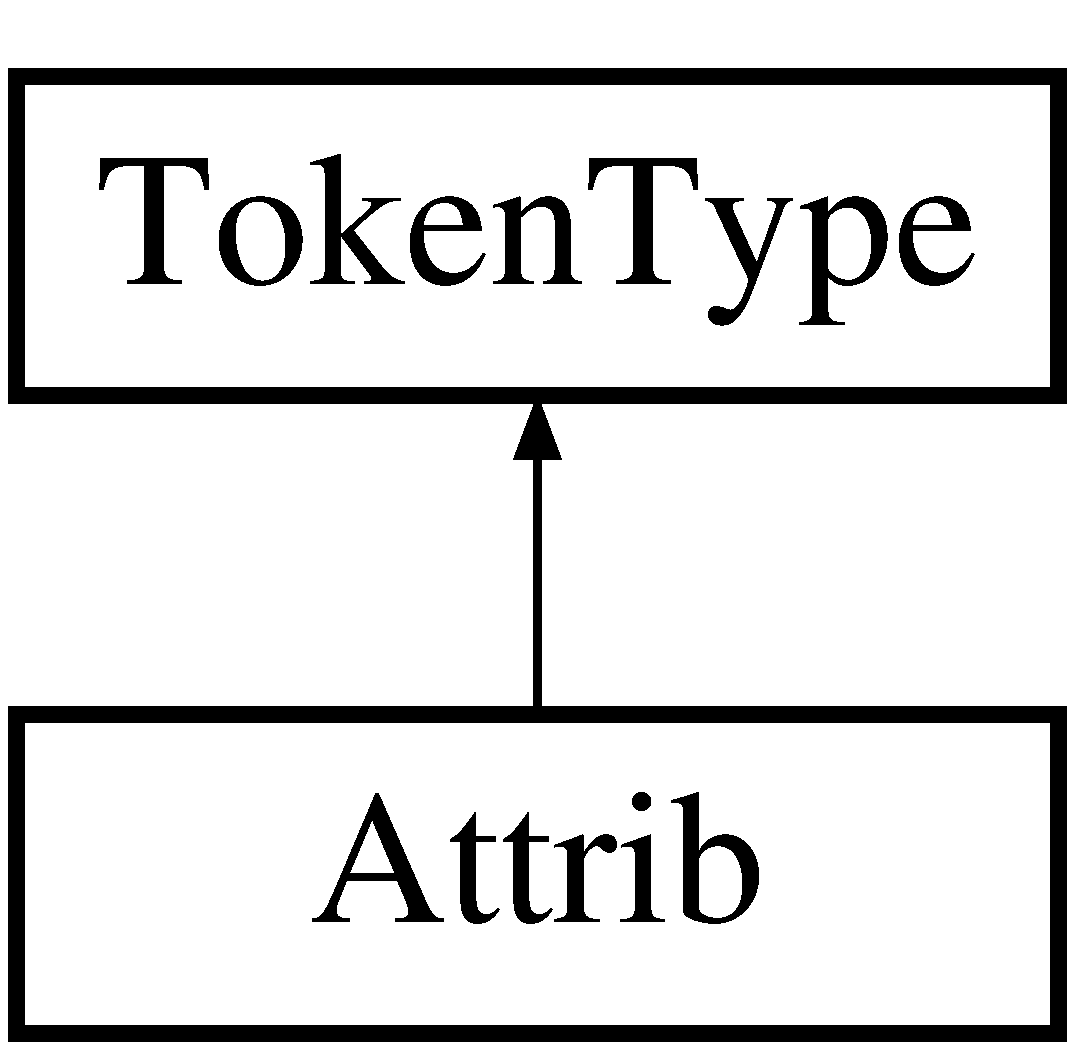
\includegraphics[height=2.000000cm]{class_attrib}
\end{center}
\end{figure}
\subsection*{Public Member Functions}
\begin{DoxyCompactItemize}
\item 
\hypertarget{class_attrib_af692b350ad68af49ac64681c1dd37190}{void {\bfseries set\-Attrib} (\hyperlink{class_token_type}{Token\-Type} $\ast$attrib)}\label{class_attrib_af692b350ad68af49ac64681c1dd37190}

\item 
\hypertarget{class_attrib_a2a795723e18599ca9da17c5af3716748}{void {\bfseries set\-Identificador} (\hyperlink{class_token_type}{Token\-Type} $\ast$var)}\label{class_attrib_a2a795723e18599ca9da17c5af3716748}

\item 
\hypertarget{class_attrib_a2ca1acd5c5ecb8f742ab288d5545bd52}{void {\bfseries set\-Expression} (\hyperlink{class_token_type}{Token\-Type} $\ast$exp)}\label{class_attrib_a2ca1acd5c5ecb8f742ab288d5545bd52}

\item 
\hypertarget{class_attrib_af4d373afcd2308d759dce8e86aeafc00}{\hyperlink{class_token_type}{Token\-Type} $\ast$ {\bfseries get\-Identificador} ()}\label{class_attrib_af4d373afcd2308d759dce8e86aeafc00}

\item 
\hypertarget{class_attrib_a2d3205310c06bec606d817f6f80d9289}{\hyperlink{class_token_type}{Token\-Type} $\ast$ {\bfseries get\-Expression} ()}\label{class_attrib_a2d3205310c06bec606d817f6f80d9289}

\end{DoxyCompactItemize}


The documentation for this class was generated from the following files\-:\begin{DoxyCompactItemize}
\item 
C\-:/\-Users/hismahil/\-Documents/\-Ruby\-Like/src/attrib.\-h\item 
C\-:/\-Users/hismahil/\-Documents/\-Ruby\-Like/src/attrib.\-cpp\end{DoxyCompactItemize}

\hypertarget{class_each}{\section{Each Class Reference}
\label{class_each}\index{Each@{Each}}
}
Inheritance diagram for Each\-:\begin{figure}[H]
\begin{center}
\leavevmode
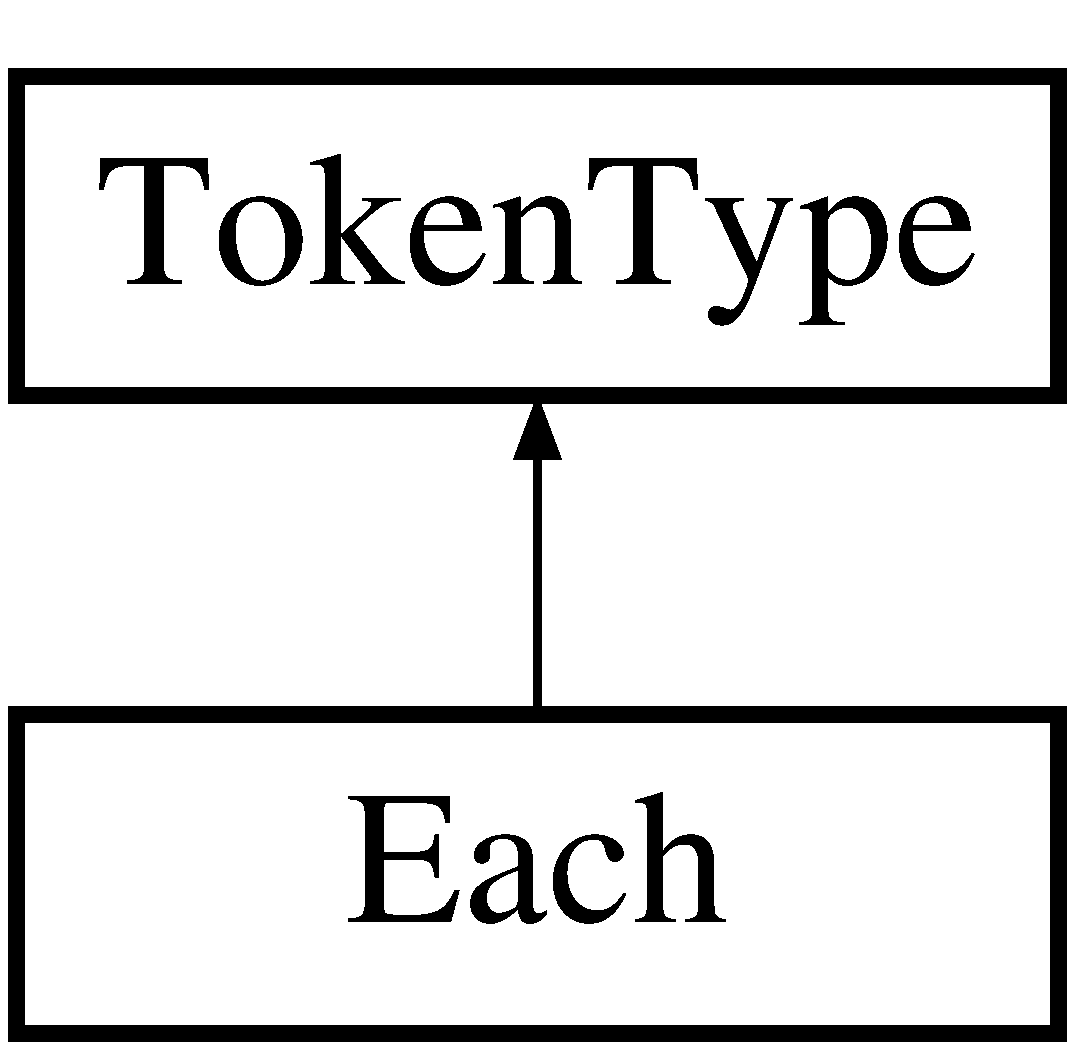
\includegraphics[height=2.000000cm]{class_each}
\end{center}
\end{figure}
\subsection*{Public Member Functions}
\begin{DoxyCompactItemize}
\item 
\hypertarget{class_each_afa02bf01ae863a66e04121ed9286ec92}{void {\bfseries set\-Each} (\hyperlink{class_token_type}{Token\-Type} $\ast$each)}\label{class_each_afa02bf01ae863a66e04121ed9286ec92}

\item 
\hypertarget{class_each_a38d48db85647d0c4bfd2b17508295dbe}{void {\bfseries set\-Expression} (\hyperlink{class_token_type}{Token\-Type} $\ast$expr)}\label{class_each_a38d48db85647d0c4bfd2b17508295dbe}

\item 
\hypertarget{class_each_aebb3578a7f206dca8cd132870d76e047}{void {\bfseries set\-Block} (\hyperlink{class_token_type}{Token\-Type} $\ast$block)}\label{class_each_aebb3578a7f206dca8cd132870d76e047}

\item 
\hypertarget{class_each_a32183537716a0503430edbc4be513286}{\hyperlink{class_token_type}{Token\-Type} $\ast$ {\bfseries get\-Expression} ()}\label{class_each_a32183537716a0503430edbc4be513286}

\item 
\hypertarget{class_each_ae1d5bcf365215c324c6f876826da0ac4}{\hyperlink{class_token_type}{Token\-Type} $\ast$ {\bfseries get\-Block} ()}\label{class_each_ae1d5bcf365215c324c6f876826da0ac4}

\end{DoxyCompactItemize}


The documentation for this class was generated from the following files\-:\begin{DoxyCompactItemize}
\item 
C\-:/\-Users/hismahil/\-Documents/\-Ruby\-Like/src/each.\-h\item 
C\-:/\-Users/hismahil/\-Documents/\-Ruby\-Like/src/each.\-cpp\end{DoxyCompactItemize}

\hypertarget{class_error}{\section{Error Class Reference}
\label{class_error}\index{Error@{Error}}
}
\subsection*{Public Member Functions}
\begin{DoxyCompactItemize}
\item 
\hypertarget{class_error_ac4ce8825ddaf31c13d3f055b643fb114}{void {\bfseries show\-Error} (const string msg, int line, int column, const string token)}\label{class_error_ac4ce8825ddaf31c13d3f055b643fb114}

\end{DoxyCompactItemize}
\subsection*{Static Public Member Functions}
\begin{DoxyCompactItemize}
\item 
\hypertarget{class_error_aace9016907bb5372c3f1309db5143c9c}{static \hyperlink{class_error}{Error} $\ast$ {\bfseries get\-Instance} ()}\label{class_error_aace9016907bb5372c3f1309db5143c9c}

\end{DoxyCompactItemize}


The documentation for this class was generated from the following files\-:\begin{DoxyCompactItemize}
\item 
C\-:/\-Users/hismahil/\-Documents/\-Ruby\-Like/src/error.\-h\item 
C\-:/\-Users/hismahil/\-Documents/\-Ruby\-Like/src/error.\-cpp\end{DoxyCompactItemize}

\hypertarget{class_file}{\section{File Class Reference}
\label{class_file}\index{File@{File}}
}
\subsection*{Public Member Functions}
\begin{DoxyCompactItemize}
\item 
\hypertarget{class_file_a1697d4d739c321a2af4097a9d139bd41}{{\bfseries File} (const string \&file\-I\-N, const string \&file\-Out)}\label{class_file_a1697d4d739c321a2af4097a9d139bd41}

\item 
\hypertarget{class_file_af1f5abf490fe288eb4a87ac0da20cc6d}{void {\bfseries open} (const string \&file\-I\-N, const string \&file\-Out)}\label{class_file_af1f5abf490fe288eb4a87ac0da20cc6d}

\item 
\hypertarget{class_file_af6794f27c00b09ee3d5ea65c16de7334}{bool {\bfseries is\-Open} ()}\label{class_file_af6794f27c00b09ee3d5ea65c16de7334}

\item 
\hypertarget{class_file_a83cbce54d6c3b8c2f417b51f6b3f488c}{void {\bfseries close} ()}\label{class_file_a83cbce54d6c3b8c2f417b51f6b3f488c}

\item 
\hypertarget{class_file_a25ace1d32d49ee9c660dd42b77944c64}{char {\bfseries read\-Char} ()}\label{class_file_a25ace1d32d49ee9c660dd42b77944c64}

\item 
\hypertarget{class_file_a30c706c71d33f7e2e2a7869ee4a82a57}{char $\ast$ {\bfseries read\-String} ()}\label{class_file_a30c706c71d33f7e2e2a7869ee4a82a57}

\item 
\hypertarget{class_file_a3c3dbdd8690d93eed7ac83cf7ebe0f7e}{void {\bfseries write\-Data} (string str)}\label{class_file_a3c3dbdd8690d93eed7ac83cf7ebe0f7e}

\end{DoxyCompactItemize}


The documentation for this class was generated from the following files\-:\begin{DoxyCompactItemize}
\item 
C\-:/\-Users/hismahil/\-Documents/\-Ruby\-Like/src/file.\-h\item 
C\-:/\-Users/hismahil/\-Documents/\-Ruby\-Like/src/file.\-cpp\end{DoxyCompactItemize}

\hypertarget{class_i_f_else}{\section{I\-F\-Else Class Reference}
\label{class_i_f_else}\index{I\-F\-Else@{I\-F\-Else}}
}
Inheritance diagram for I\-F\-Else\-:\begin{figure}[H]
\begin{center}
\leavevmode
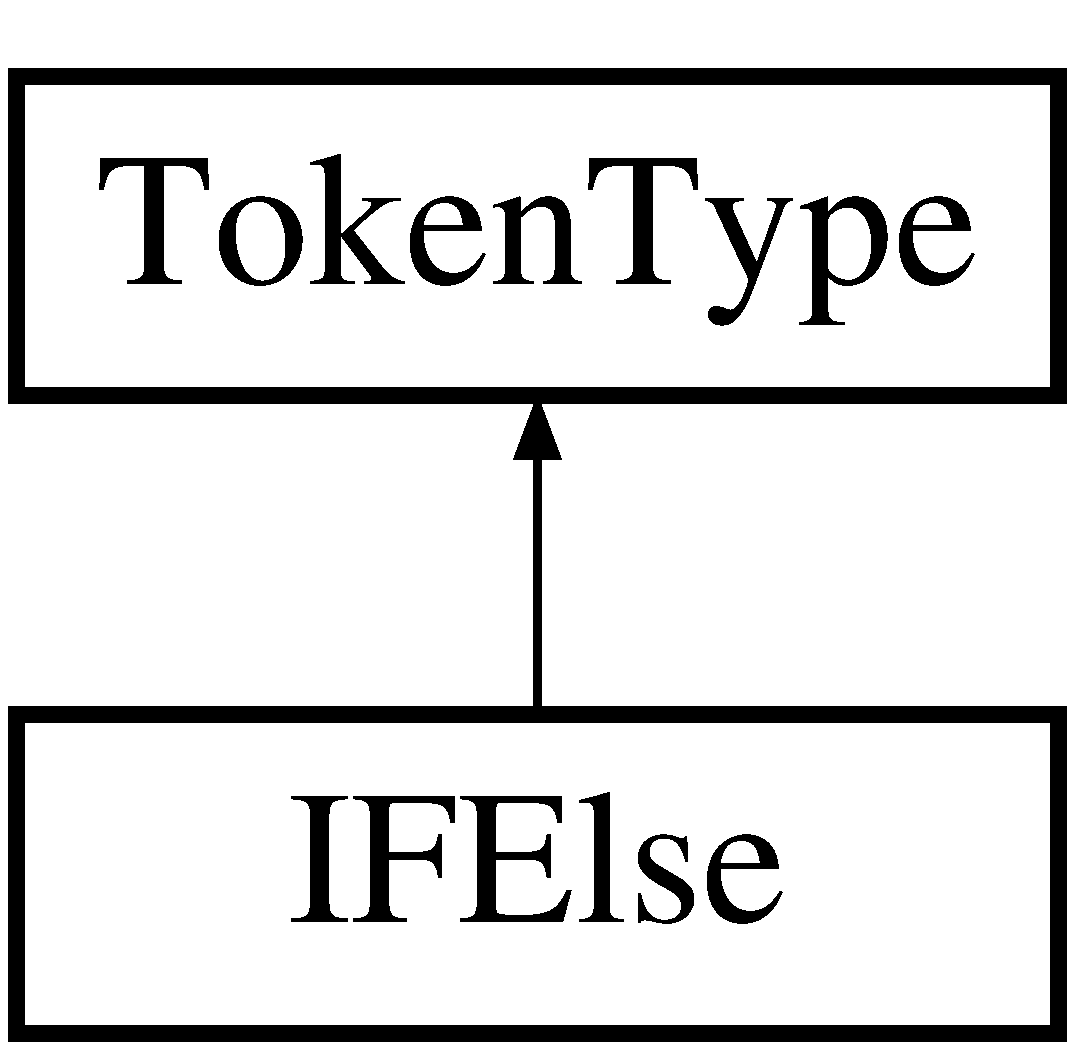
\includegraphics[height=2.000000cm]{class_i_f_else}
\end{center}
\end{figure}
\subsection*{Public Member Functions}
\begin{DoxyCompactItemize}
\item 
\hypertarget{class_i_f_else_a141bc736d3a84b62755583ef66b0e06e}{void {\bfseries set\-I\-F} (\hyperlink{class_token_type}{Token\-Type} $\ast$\-\_\-if)}\label{class_i_f_else_a141bc736d3a84b62755583ef66b0e06e}

\item 
\hypertarget{class_i_f_else_a5a8044af71dbc6183923611367146ed8}{void {\bfseries set\-Expression} (\hyperlink{class_token_type}{Token\-Type} $\ast$expr)}\label{class_i_f_else_a5a8044af71dbc6183923611367146ed8}

\item 
\hypertarget{class_i_f_else_a3a0f6dec06c70cd36a9e584ea59ac590}{void {\bfseries set\-Block\-I\-F} (\hyperlink{class_token_type}{Token\-Type} $\ast$block)}\label{class_i_f_else_a3a0f6dec06c70cd36a9e584ea59ac590}

\item 
\hypertarget{class_i_f_else_af899b6a6fdf1d242a3a6fcb82c2a7bed}{void {\bfseries set\-Else\-Block} (\hyperlink{class_token_type}{Token\-Type} $\ast$block)}\label{class_i_f_else_af899b6a6fdf1d242a3a6fcb82c2a7bed}

\item 
\hypertarget{class_i_f_else_ab57532ebd0f594e6b63f177e2048e4e6}{\hyperlink{class_token_type}{Token\-Type} $\ast$ {\bfseries get\-Expression} ()}\label{class_i_f_else_ab57532ebd0f594e6b63f177e2048e4e6}

\item 
\hypertarget{class_i_f_else_a823b002825a5b52e53d2cfb00bfccbc3}{\hyperlink{class_token_type}{Token\-Type} $\ast$ {\bfseries get\-Block\-I\-F} ()}\label{class_i_f_else_a823b002825a5b52e53d2cfb00bfccbc3}

\item 
\hypertarget{class_i_f_else_a637b37e809e0e9abd475689eb03d5334}{\hyperlink{class_token_type}{Token\-Type} $\ast$ {\bfseries get\-Else\-Block} ()}\label{class_i_f_else_a637b37e809e0e9abd475689eb03d5334}

\end{DoxyCompactItemize}


The documentation for this class was generated from the following files\-:\begin{DoxyCompactItemize}
\item 
C\-:/\-Users/hismahil/\-Documents/\-Ruby\-Like/src/ifelse.\-h\item 
C\-:/\-Users/hismahil/\-Documents/\-Ruby\-Like/src/ifelse.\-cpp\end{DoxyCompactItemize}

\hypertarget{class_lex}{\section{Lex Class Reference}
\label{class_lex}\index{Lex@{Lex}}
}
\subsection*{Public Member Functions}
\begin{DoxyCompactItemize}
\item 
\hypertarget{class_lex_a813e096370b67b475023a586632266e3}{void {\bfseries start\-Lex} (\hyperlink{class_file}{File} \&file)}\label{class_lex_a813e096370b67b475023a586632266e3}

\item 
\hypertarget{class_lex_a8b6f8ab084b0f9e61d5df289c20f18e6}{\hyperlink{class_token_type}{Token\-Type} $\ast$ {\bfseries get\-Token} ()}\label{class_lex_a8b6f8ab084b0f9e61d5df289c20f18e6}

\end{DoxyCompactItemize}


The documentation for this class was generated from the following files\-:\begin{DoxyCompactItemize}
\item 
C\-:/\-Users/hismahil/\-Documents/\-Ruby\-Like/src/lex.\-h\item 
C\-:/\-Users/hismahil/\-Documents/\-Ruby\-Like/src/lex.\-cpp\end{DoxyCompactItemize}

\hypertarget{class_operator}{\section{Operator Class Reference}
\label{class_operator}\index{Operator@{Operator}}
}
Inheritance diagram for Operator\-:\begin{figure}[H]
\begin{center}
\leavevmode
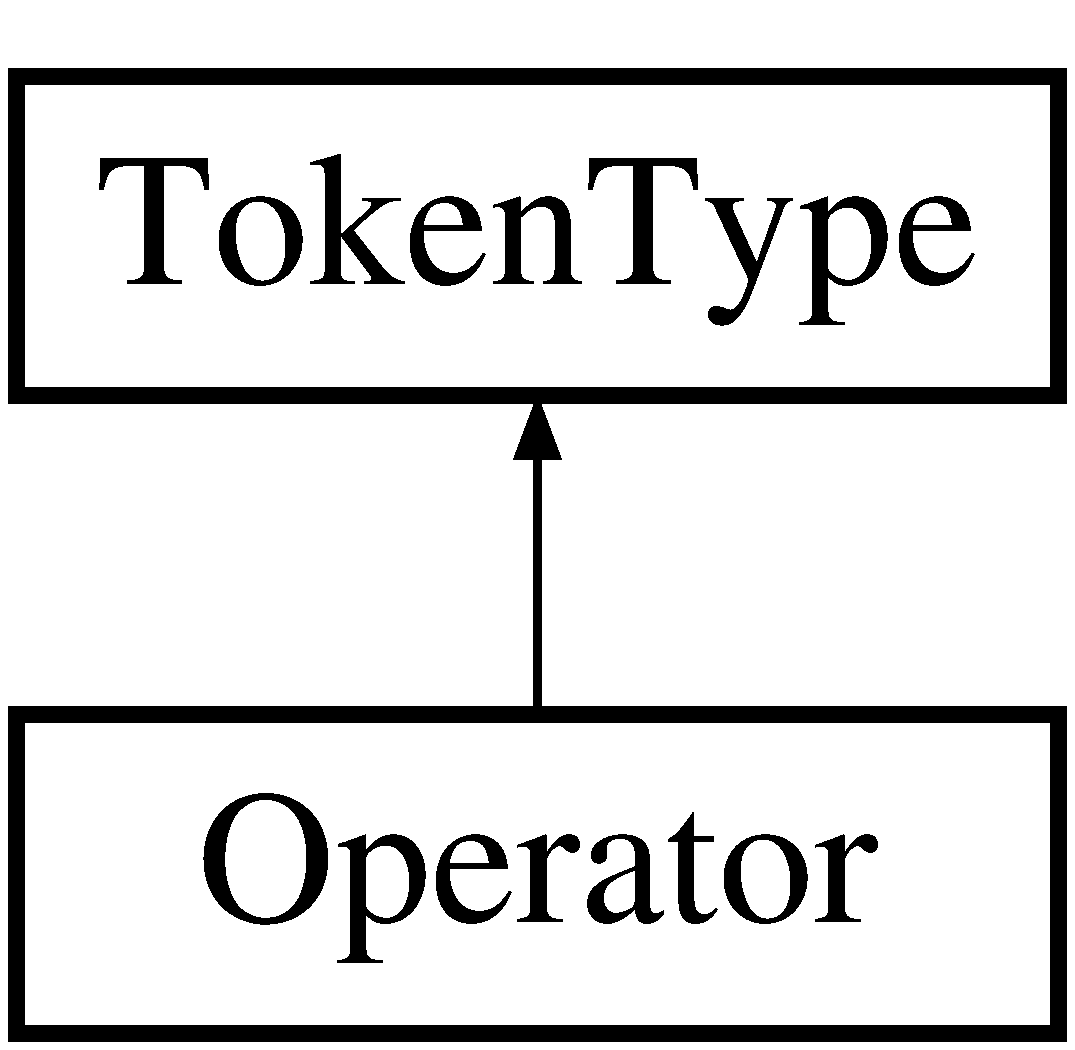
\includegraphics[height=2.000000cm]{class_operator}
\end{center}
\end{figure}
\subsection*{Public Member Functions}
\begin{DoxyCompactItemize}
\item 
\hypertarget{class_operator_aa115e40a7b4bb634472e28a1daad410f}{void {\bfseries set\-Operator} (\hyperlink{class_token_type}{Token\-Type} $\ast$opr)}\label{class_operator_aa115e40a7b4bb634472e28a1daad410f}

\item 
\hypertarget{class_operator_ac37299186464e9dfe8557391e679fbf6}{void {\bfseries set\-Left} (\hyperlink{class_token_type}{Token\-Type} $\ast$left)}\label{class_operator_ac37299186464e9dfe8557391e679fbf6}

\item 
\hypertarget{class_operator_a79b4dd10947277fa71a3e57508d5cf4f}{void {\bfseries set\-Right} (\hyperlink{class_token_type}{Token\-Type} $\ast$right)}\label{class_operator_a79b4dd10947277fa71a3e57508d5cf4f}

\item 
\hypertarget{class_operator_acb61fc8562334b90eed92b067d603188}{\hyperlink{class_token_type}{Token\-Type} $\ast$ {\bfseries get\-Left} ()}\label{class_operator_acb61fc8562334b90eed92b067d603188}

\item 
\hypertarget{class_operator_a7a32321aaa7c0b8f54101f46361b20fd}{\hyperlink{class_token_type}{Token\-Type} $\ast$ {\bfseries get\-Right} ()}\label{class_operator_a7a32321aaa7c0b8f54101f46361b20fd}

\end{DoxyCompactItemize}


The documentation for this class was generated from the following files\-:\begin{DoxyCompactItemize}
\item 
C\-:/\-Users/hismahil/\-Documents/\-Ruby\-Like/src/operator.\-h\item 
C\-:/\-Users/hismahil/\-Documents/\-Ruby\-Like/src/operator.\-cpp\end{DoxyCompactItemize}

\hypertarget{class_producer_list}{\section{Producer\-List Class Reference}
\label{class_producer_list}\index{Producer\-List@{Producer\-List}}
}
\subsection*{Public Member Functions}
\begin{DoxyCompactItemize}
\item 
\hypertarget{class_producer_list_a3e17fb470a8d0079bcceb7c82e1ad45a}{void {\bfseries insert} (\hyperlink{class_token_type}{Token\-Type} $\ast$i)}\label{class_producer_list_a3e17fb470a8d0079bcceb7c82e1ad45a}

\item 
\hypertarget{class_producer_list_a0cb8b0344e7bd61da72b2e14f27ee12e}{\hyperlink{class_token_type}{Token\-Type} $\ast$ {\bfseries get\-Token\-Of\-List} (string prod)}\label{class_producer_list_a0cb8b0344e7bd61da72b2e14f27ee12e}

\item 
\hypertarget{class_producer_list_a6d34f625be27fbe3ba9851f9dd03e04b}{bool {\bfseries is\-Producer} (string prod)}\label{class_producer_list_a6d34f625be27fbe3ba9851f9dd03e04b}

\item 
\hypertarget{class_producer_list_a33ea5b4211d1709d8da4116a1630f8ab}{string {\bfseries get\-String} ()}\label{class_producer_list_a33ea5b4211d1709d8da4116a1630f8ab}

\item 
\hypertarget{class_producer_list_add7f3ea66a2ff4a8dc911b39a2212e98}{void {\bfseries show\-Values} ()}\label{class_producer_list_add7f3ea66a2ff4a8dc911b39a2212e98}

\item 
\hypertarget{class_producer_list_af3744891c313fc968e28108003e22bfa}{void {\bfseries show\-Value\-At} (int index)}\label{class_producer_list_af3744891c313fc968e28108003e22bfa}

\end{DoxyCompactItemize}
\subsection*{Static Public Member Functions}
\begin{DoxyCompactItemize}
\item 
\hypertarget{class_producer_list_aada51af5836a6086df9f86512c2e1963}{static \hyperlink{class_producer_list}{Producer\-List} $\ast$ {\bfseries get\-Instance} ()}\label{class_producer_list_aada51af5836a6086df9f86512c2e1963}

\end{DoxyCompactItemize}


The documentation for this class was generated from the following files\-:\begin{DoxyCompactItemize}
\item 
C\-:/\-Users/hismahil/\-Documents/\-Ruby\-Like/src/producerlist.\-h\item 
C\-:/\-Users/hismahil/\-Documents/\-Ruby\-Like/src/producerlist.\-cpp\end{DoxyCompactItemize}

\hypertarget{class_semantic}{\section{Semantic Class Reference}
\label{class_semantic}\index{Semantic@{Semantic}}
}
\subsection*{Public Member Functions}
\begin{DoxyCompactItemize}
\item 
\hypertarget{class_semantic_a2f5269187e39b421d64a62ba500d1d31}{void {\bfseries parsing} ()}\label{class_semantic_a2f5269187e39b421d64a62ba500d1d31}

\end{DoxyCompactItemize}


The documentation for this class was generated from the following files\-:\begin{DoxyCompactItemize}
\item 
C\-:/\-Users/hismahil/\-Documents/\-Ruby\-Like/src/semantic.\-h\item 
C\-:/\-Users/hismahil/\-Documents/\-Ruby\-Like/src/semantic.\-cpp\end{DoxyCompactItemize}

\hypertarget{class_syntactic}{\section{Syntactic Class Reference}
\label{class_syntactic}\index{Syntactic@{Syntactic}}
}
\subsection*{Public Member Functions}
\begin{DoxyCompactItemize}
\item 
\hypertarget{class_syntactic_ac94e5b2e82e2c0d2ad751b3f5ada8061}{{\bfseries Syntactic} (\hyperlink{class_lex}{Lex} $\ast$lex)}\label{class_syntactic_ac94e5b2e82e2c0d2ad751b3f5ada8061}

\item 
\hypertarget{class_syntactic_aa853bd9d18eee01a03dab6752ae215aa}{void {\bfseries parser} ()}\label{class_syntactic_aa853bd9d18eee01a03dab6752ae215aa}

\item 
\hypertarget{class_syntactic_aeab5765ad28f7a887885b84eab428016}{void {\bfseries show} ()}\label{class_syntactic_aeab5765ad28f7a887885b84eab428016}

\end{DoxyCompactItemize}


The documentation for this class was generated from the following files\-:\begin{DoxyCompactItemize}
\item 
C\-:/\-Users/hismahil/\-Documents/\-Ruby\-Like/src/syntactic.\-h\item 
C\-:/\-Users/hismahil/\-Documents/\-Ruby\-Like/src/syntactic.\-cpp\end{DoxyCompactItemize}

\hypertarget{class_table_symbol}{\section{Table\-Symbol Class Reference}
\label{class_table_symbol}\index{Table\-Symbol@{Table\-Symbol}}
}
\subsection*{Public Member Functions}
\begin{DoxyCompactItemize}
\item 
\hypertarget{class_table_symbol_ade8b6278058048d48c1f94615b367269}{bool {\bfseries find\-Symbol} (string str)}\label{class_table_symbol_ade8b6278058048d48c1f94615b367269}

\item 
\hypertarget{class_table_symbol_affae95bc57362eb5a9b43a0f4b2ff1d3}{void {\bfseries show\-Keys\-Values} ()}\label{class_table_symbol_affae95bc57362eb5a9b43a0f4b2ff1d3}

\end{DoxyCompactItemize}
\subsection*{Static Public Member Functions}
\begin{DoxyCompactItemize}
\item 
\hypertarget{class_table_symbol_a1d511bbd611e740b719e614e9a30d491}{static \hyperlink{class_table_symbol}{Table\-Symbol} $\ast$ {\bfseries get\-Instance} ()}\label{class_table_symbol_a1d511bbd611e740b719e614e9a30d491}

\end{DoxyCompactItemize}


The documentation for this class was generated from the following files\-:\begin{DoxyCompactItemize}
\item 
C\-:/\-Users/hismahil/\-Documents/\-Ruby\-Like/src/tablesymbol.\-h\item 
C\-:/\-Users/hismahil/\-Documents/\-Ruby\-Like/src/tablesymbol.\-cpp\end{DoxyCompactItemize}

\hypertarget{class_t_list}{\section{T\-List Class Reference}
\label{class_t_list}\index{T\-List@{T\-List}}
}
Inheritance diagram for T\-List\-:\begin{figure}[H]
\begin{center}
\leavevmode
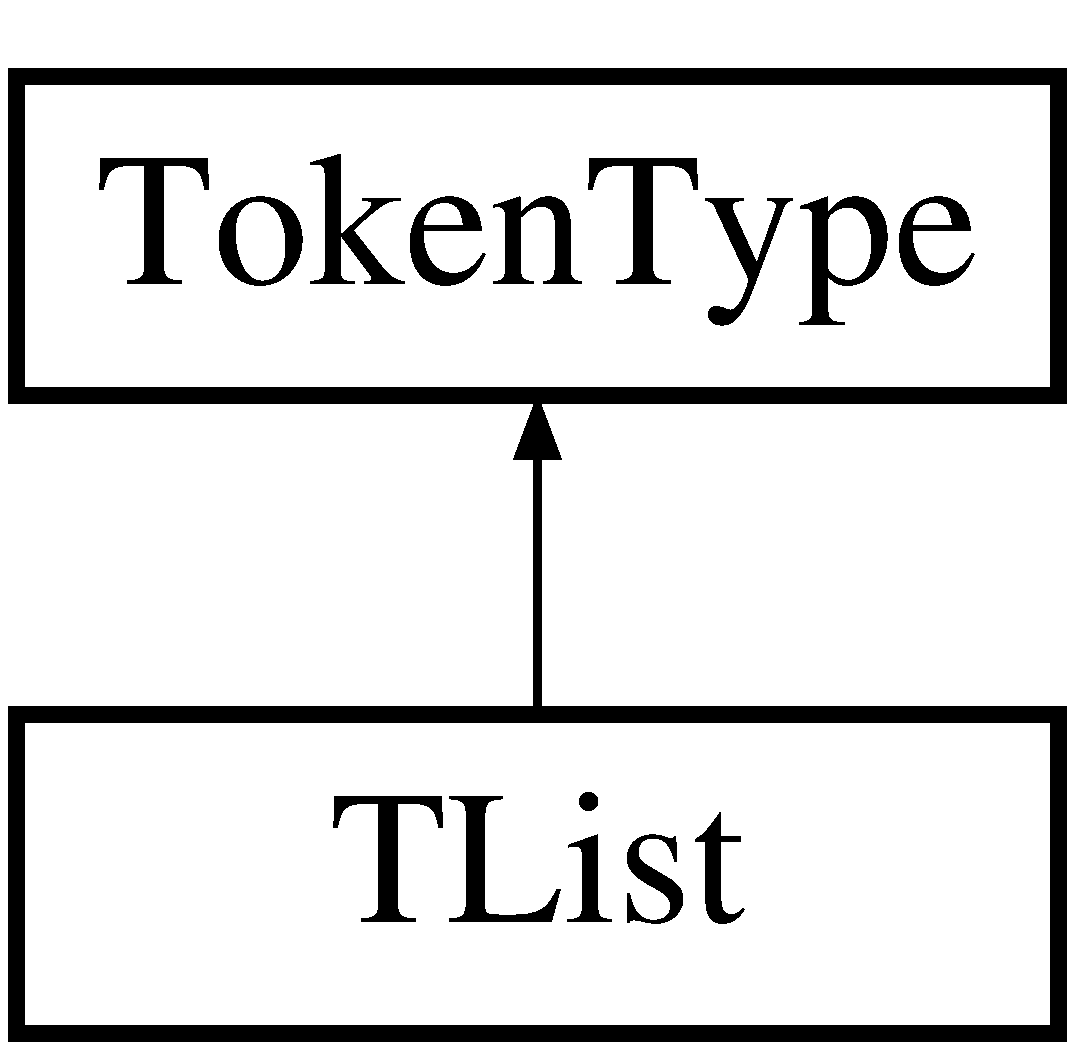
\includegraphics[height=2.000000cm]{class_t_list}
\end{center}
\end{figure}
\subsection*{Public Member Functions}
\begin{DoxyCompactItemize}
\item 
\hypertarget{class_t_list_a5264d60dba1001725d5d5f17d1482ce5}{void {\bfseries set\-List} (\hyperlink{class_token_type}{Token\-Type} $\ast$list)}\label{class_t_list_a5264d60dba1001725d5d5f17d1482ce5}

\item 
\hypertarget{class_t_list_a5a5470e91edefc47c0505579e3fecda9}{void {\bfseries insere} (\hyperlink{class_token_type}{Token\-Type} $\ast$token)}\label{class_t_list_a5a5470e91edefc47c0505579e3fecda9}

\item 
\hypertarget{class_t_list_aed59c80477b7c0c85a1f5d5a8b11bcc7}{\hyperlink{class_token_type}{Token\-Type} $\ast$ {\bfseries get\-Index\-Of} (int index)}\label{class_t_list_aed59c80477b7c0c85a1f5d5a8b11bcc7}

\item 
\hypertarget{class_t_list_a94f03c8ae61a506d8d29ca649538b209}{void {\bfseries show\-Itens} ()}\label{class_t_list_a94f03c8ae61a506d8d29ca649538b209}

\end{DoxyCompactItemize}


The documentation for this class was generated from the following files\-:\begin{DoxyCompactItemize}
\item 
C\-:/\-Users/hismahil/\-Documents/\-Ruby\-Like/src/tlist.\-h\item 
C\-:/\-Users/hismahil/\-Documents/\-Ruby\-Like/src/tlist.\-cpp\end{DoxyCompactItemize}

\hypertarget{class_token_type}{\section{Token\-Type Class Reference}
\label{class_token_type}\index{Token\-Type@{Token\-Type}}
}
Inheritance diagram for Token\-Type\-:\begin{figure}[H]
\begin{center}
\leavevmode
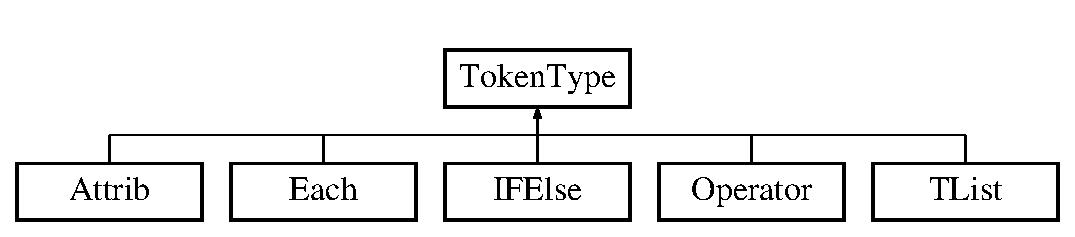
\includegraphics[height=2.000000cm]{class_token_type}
\end{center}
\end{figure}
\subsection*{Public Member Functions}
\begin{DoxyCompactItemize}
\item 
\hypertarget{class_token_type_a3b011053a11e2d82f58d2046702a1257}{void {\bfseries set\-Classe} (int classe)}\label{class_token_type_a3b011053a11e2d82f58d2046702a1257}

\item 
\hypertarget{class_token_type_ac7ecfb01f9d72e23d6dc3d6a8f081a80}{void {\bfseries set\-Token} (string repr)}\label{class_token_type_ac7ecfb01f9d72e23d6dc3d6a8f081a80}

\item 
\hypertarget{class_token_type_a93e22d1c0424d1edf8f6ee8e66d7ff31}{void {\bfseries set\-Line} (int line)}\label{class_token_type_a93e22d1c0424d1edf8f6ee8e66d7ff31}

\item 
\hypertarget{class_token_type_a1b19294195be56652d1d37f736462277}{void {\bfseries set\-Column} (int column)}\label{class_token_type_a1b19294195be56652d1d37f736462277}

\item 
\hypertarget{class_token_type_a143e63aff1ffc82e11f42eb23e5bd448}{void {\bfseries set\-Next} (\hyperlink{class_token_type}{Token\-Type} $\ast$no)}\label{class_token_type_a143e63aff1ffc82e11f42eb23e5bd448}

\item 
\hypertarget{class_token_type_a371ad064991e873616d98fb7a388f00a}{void {\bfseries set\-Type} (int type)}\label{class_token_type_a371ad064991e873616d98fb7a388f00a}

\item 
\hypertarget{class_token_type_ac64dbb3f1f493c598bd629631f6e3274}{int {\bfseries get\-Classe} ()}\label{class_token_type_ac64dbb3f1f493c598bd629631f6e3274}

\item 
\hypertarget{class_token_type_a8a899b8b6f05074c8330ec54849ff3f8}{string {\bfseries get\-Token} ()}\label{class_token_type_a8a899b8b6f05074c8330ec54849ff3f8}

\item 
\hypertarget{class_token_type_aee7a165d0de8d9f58a16f96e987705f4}{int {\bfseries get\-Line} ()}\label{class_token_type_aee7a165d0de8d9f58a16f96e987705f4}

\item 
\hypertarget{class_token_type_a34ab252ea0332496b0605acb6cab450f}{int {\bfseries get\-Column} ()}\label{class_token_type_a34ab252ea0332496b0605acb6cab450f}

\item 
\hypertarget{class_token_type_a38ce58f3163b029f4788ca1ad025fc04}{int {\bfseries get\-Type} ()}\label{class_token_type_a38ce58f3163b029f4788ca1ad025fc04}

\item 
\hypertarget{class_token_type_ad3ebcefc31023426c1e13d08d348bf34}{\hyperlink{class_token_type}{Token\-Type} $\ast$ {\bfseries get\-Next} ()}\label{class_token_type_ad3ebcefc31023426c1e13d08d348bf34}

\end{DoxyCompactItemize}


The documentation for this class was generated from the following files\-:\begin{DoxyCompactItemize}
\item 
C\-:/\-Users/hismahil/\-Documents/\-Ruby\-Like/src/tokentype.\-h\item 
C\-:/\-Users/hismahil/\-Documents/\-Ruby\-Like/src/tokentype.\-cpp\end{DoxyCompactItemize}

%--- End generated contents ---

% Index
\newpage
\phantomsection
\addcontentsline{toc}{part}{Index}
\printindex

\end{document}
